\subsection{Where the classical routes stop}
\label{sec:walls}

Evaluating the inequalities of Section~\ref{sec:framework} for the budgets of Table~\ref{tab:params} gives the first failing $N$ of each route (Table~\ref{tab:walls}). Full-state storage fails by a count, early on the grid and later in a compressed basis. The tensor-network wall is Eq.~\eqref{eq:Nstar} evaluated on the entropy of Section~\ref{sec:larger}: under the three scenarios for the one-particle entropy it lies on the grid between $N=\num{wall_pess_grid}$ (entropy keeps growing) and $N=\num{wall_opt_grid}$ (saturated at its $N=\num{Nmax_measured}$ value) \stC{}, with the compute budget binding first (Fig.~\ref{fig:walls}). Since most of that entanglement is static (Section~\ref{sec:static}), the wall prices the representation of the evolved state, not the task.

\begin{table}[ht]
\centering
\footnotesize
\caption{Where each classical route first fails (first failing $N$) for the budgets of Table~\ref{tab:params}. Exact diagonalization is an exact count; the tensor-network rows evaluate the cost model of Prop.~\ref{prop:tn} on the graph law of Section~\ref{sec:larger} under three assumptions about the one-particle entropy beyond the largest simulated $N$. In parentheses: the same with the numerical Schmidt rank $\chi(10^{-3})$ charged instead of $2^{S}$, at the ratio measured at $N=6$ ($+\num{chi_shift}$ bits).}
\label{tab:walls}
\begin{tabular}{L{4.0cm}L{5.3cm}cc}
\toprule
Route & Assumption & grid, $d=\num{d_grid}$ & modes, $d=\num{d_mode}$ \\
\midrule
Exact diagonalization, distinguishable & exact count & 4 & 8 \\
Exact diagonalization, bosonic & exact count & 4 & 17 \\
\midrule
Tensor networks & entropy keeps growing at the $N=4\to6$ rate & 13 (7) & 18 (13) \\
Tensor networks & one-particle entropy saturates (fit) & 15 (7) & 25 (16) \\
Tensor networks & one-particle entropy saturated at $N=6$ & 16 (7) & 27 (17) \\
\bottomrule
\end{tabular}
\end{table}


\begin{figure}[t]
\centering
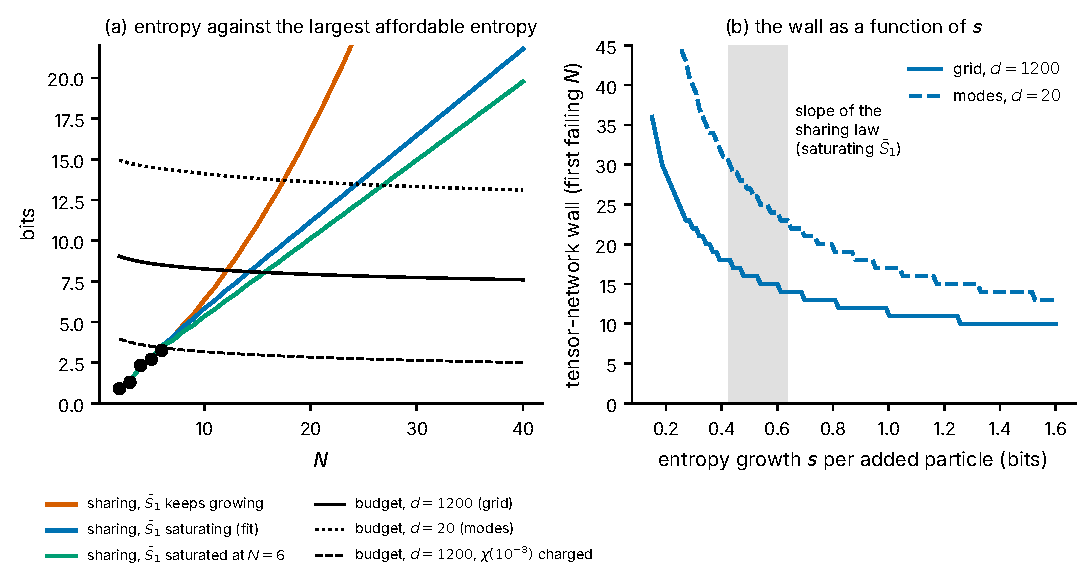
\includegraphics[width=\textwidth]{figures/fig_walls.pdf}
\caption{\textbf{The tensor-network wall.} (a) The central-cut entropy under the three scenarios of Section~\ref{sec:larger} against the largest entropy that the memory and compute budgets of Table~\ref{tab:params} allow (grid and mode basis;
dashed: grid budget when the numerical Schmidt rank $\chi(10^{-3})$ is charged instead of $2^{S}$, Section~\ref{sec:seed}). The wall is the first crossing. (b) The wall for a constant growth $s$ per added particle anchored at the last simulated $N$ (Eq.~\eqref{eq:Nflop}); the grey band is the asymptotic slope
of the sharing law. Computed from the measured entropies and the budgets of Table~\ref{tab:params}.}
\label{fig:walls}
\end{figure}

A matrix-product state was also run (density-matrix-renormalization-group start, two-site time-dependent variational evolution) as an independent check of the counting model. It reproduces the exact entropies to a few hundredths of a bit or better (Table~\ref{tab:mps}, Fig.~\ref{fig:tn}a) but is slower than the exact code at the sizes tried, so it reaches only $N\le5$ and extends no data. Two corrections to the model go in opposite directions, and neither is converged. The numerical Schmidt rank $\chi(10^{-3})$ exceeds $2^{S}$ by a factor that grows with $N$ and $k$ (Fig.~\ref{fig:tn}b); charging it at the ratio measured at $N=6$ adds $\num{chi_shift}$ bits and moves the grid wall to the values in parentheses in Table~\ref{tab:walls}. Charging the central bond on every bond, and the natural order instead of a better tree, overstates the cost (Lemma~\ref{lem:chord}). The wall moves by only $\log_2f/(3s)$ particles for a factor $f$ in the budget (Eq.~\eqref{eq:Nflop}), so the lower edge of the window is the soft quantity of the bounds, and Fig.~\ref{fig:regime} shades it rather than cutting it. The measured cost per step is nearly flat in $\chi$ at these sizes (Fig.~\ref{fig:tn}c), so the model's prefactor is a lower bound and has not been tested where the bond cap matters.

\begin{table}[ht]
\centering
\small
\caption{A matrix-product state (density-matrix-renormalization-group start, two-site time-dependent variational evolution) against the exact propagation of the same case, correlated start, resonant tilt, window $T$ (shorter than $T=\num{Tprot}$ so that the exact run is cheap). $S_{\rm cen}$: central-bond entropy (bits); $\max\Delta S$: largest difference over every cut both methods measured and every snapshot; $\chi_{10^{-3}}$: numerical Schmidt rank of the central bond (at odd $N$, of the two central bonds the one with the larger entropy); $\chi_{\max}$: cap on the bond dimension (binding where $\chi_{10^{-6}}$ of the MPS equals it). Last column: wall time of the MPS over that of the exact code (a shared four-core machine; an order of magnitude only). The $k=6$ rows validate the method in a saturated basis; the $k=12$ row is capped at $\chi_{\max}$ and its $S_{\rm cen}$ is $\num{tn_k12_dSc}$ bit below the exact value.}
\label{tab:mps}
\begin{tabular}{rrrrrrrrr}
\toprule
$N$ & $k$ & $T$ & $\chi_{\max}$ & $S_{\rm cen}$ MPS & $S_{\rm cen}$ exact & $\max\Delta S$ & $\chi_{10^{-3}}$ MPS / exact & slower by \\
\midrule
3 & 6 & 60 & 120 & 1.7332 & 1.7332 & \ensuremath{1.8\times10^{-5}} & 5 / 5 & 43$\times$ \\
4 & 6 & 60 & 120 & 2.4444 & 2.4449 & \ensuremath{5.9\times10^{-4}} & 18 / 18 & 76$\times$ \\
5 & 6 & 40 & 100 & 3.9603 & 3.9602 & \ensuremath{1.8\times10^{-3}} & 32 / 32 & 74$\times$ \\
4 & 12 & 40 & 64 & 2.2431 & 2.2640 & \ensuremath{2.8\times10^{-2}} & 32 / 35 & 146$\times$ \\
\bottomrule
\end{tabular}
\end{table}


\begin{figure}[t]
\centering
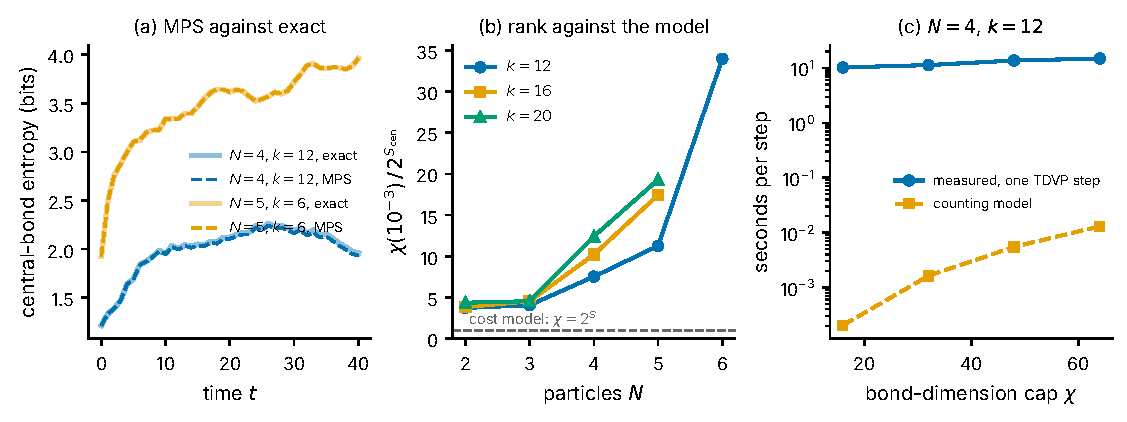
\includegraphics[width=\textwidth]{figures/fig_tn.pdf}
\caption{\textbf{What the matrix-product state measured.} (a) Central-bond entropy against time, matrix-product state (dashed) and exact (solid). (b) The numerical Schmidt rank $\chi(10^{-3})$ of the central bond in units of $2^{S_{\rm cen}}$, the value charged by the cost model, for the stored exact runs at $T=\num{Tprot}$. (c) Seconds per two-site step at $N=4$, $k=12$, measured, against the operation count of the counting model at the measured matrix-multiplication rate of the same machine.}
\label{fig:tn}
\end{figure}

By Eq.~\eqref{eq:scrit} the window at the simulated mass is non-empty if the growth per particle beyond $N=\num{Nmax_measured}$ exceeds $s_{\rm crit}$ (Table~\ref{tab:scrit}): existence is robust on the grid and marginal in the mode basis, and it refers to the entropy-based wall, which prices static entanglement, so it does not carry over to the dynamics.

\begin{table}[ht]
\centering
\small
\caption{Does a window exist at all? The growth per added particle $s_{\rm crit}$ (bits, Eq.~\eqref{eq:scrit}) that the central cut must exceed beyond $N=\num{Nmax_measured}$ for the window at the simulated mass to be non-empty with its upper end at $N_{\rm hi}$, against what the data give: the asymptotic slopes of the sharing law (saturated and saturating $\bar S_1$) and the last measured step.}
\label{tab:scrit}
\begin{tabular}{lccc}
\toprule
& $N_{\rm hi}=24$ & $N_{\rm hi}=40$ & $N_{\rm hi}=88$ \\
\midrule
$s_{\rm crit}$, grid & 0.25 & 0.13 & 0.05 \\
$s_{\rm crit}$, $20$-mode basis & 0.58 & 0.30 & 0.12 \\
\midrule
sharing-law slope, $\bar S_1$ saturated & \multicolumn{3}{c}{0.48} \\
sharing-law slope, $\bar S_1$ saturating (fit) & \multicolumn{3}{c}{0.53} \\
last measured step & \multicolumn{3}{c}{0.54} \\
\bottomrule
\end{tabular}
\end{table}


Imaginary-time Monte Carlo (Section~\ref{sec:mc}) is not excluded. Table~\ref{tab:mc} tests the picture it relies on: where the doublet test passes ($N=2,3$ and $N=4$, $k=20$) a prediction from the splitting alone is adequate; elsewhere the signal has several frequencies, and a prediction would need a handful of levels and weights, not one splitting.

\begin{table}[ht]
\centering
\small
\caption{How many frequencies describe the signal. Residual, in units of the standard deviation of $\langle\Op\rangle(t)$, of the best single cosine at the splitting $\Delta E$ of the gated pair (what imaginary-time Monte Carlo of the splitting would predict) and at a free frequency; and the number of cosines of a free fit (greedy pursuit with joint refit of the amplitudes) needed for a residual below $20\%$, $10\%$ and $5\%$ ($>8$: not reached with up to eight cosines). Where the doublet test passes ($N=2,3$ and $N=4$, $k=20$) a splitting-based prediction is adequate; elsewhere the gated splitting explains none of the signal, and the number of cosines tends to grow with $N$ and to fall with $k$ (the basis is not converged at $N=5,6$). At $N=5$, $k=20$ the best free cosine sits at $\num{cr_N5_k20_wratio}$ times $\Delta E$.}
\label{tab:mc}
\begin{tabular}{lcccccc}
\toprule
 & \multicolumn{2}{c}{residual of one cosine} & \multicolumn{3}{c}{cosines for residual below} \\
\cmidrule(lr){2-3}\cmidrule(lr){4-6}
case & at $\Delta E$ & free & $20\%$ & $10\%$ & $5\%$ \\
\midrule
$N=2$, all $k$ & 0.10--0.14 & 0.10--0.13 & 1 & 1--2 & 3 \\
$N=3$, 6 basis sizes & 0.12--0.15 & 0.12--0.15 & 1 & 2--3 & 3--5 \\
$N=4$, $k=12$ & 1.00 & 0.72 & 4 & 7 & \ensuremath{>}8 \\
$N=4$, $k=16$ & 1.00 & 0.41 & 3 & 5 & 7 \\
$N=4$, $k=20$ & 0.18 & 0.17 & 1 & 3 & 5 \\
$N=5$, $k=12$ & 0.85 & 0.74 & 3 & 8 & \ensuremath{>}8 \\
$N=5$, $k=16$ & 1.00 & 0.48 & 3 & 4 & \ensuremath{>}8 \\
$N=5$, $k=20$ & 1.00 & 0.24 & 2 & 4 & 8 \\
$N=6$, $k=12$ & 0.99 & 0.55 & 4 & \ensuremath{>}8 & \ensuremath{>}8 \\
\bottomrule
\end{tabular}
\end{table}

